%%%%%%%%%%%%%%%%%%%%%%%%%%%%%%%%%%%%%%%%%%%%%%%
%%% Template for lab reports used at STIMA
%%%%%%%%%%%%%%%%%%%%%%%%%%%%%%%%%%%%%%%%%%%%%%%

%%%%%%%%%%%%%%%%%%%%%%%%%%%%%% Sets the document class for the document
% Openany is added to remove the book style of starting every new chapter on an odd page (not needed for reports)
\documentclass[10pt,english, openany]{book}

%%%%%%%%%%%%%%%%%%%%%%%%%%%%%% Loading packages that alter the style
\usepackage[]{graphicx}
% \documentclass[11pt, a4paper]{article}
\usepackage{graphicx}
\usepackage{amsmath}

\usepackage{amsmath}
\usepackage{listings}
\usepackage[]{color}
\usepackage{alltt}
\usepackage{amsmath, amssymb}
\usepackage[T1]{fontenc}
\usepackage[utf8]{inputenc}
\usepackage{lipsum}
\setcounter{secnumdepth}{3}
\setcounter{tocdepth}{3}
\setlength{\parskip}{\smallskipamount}
\setlength{\parindent}{0pt}

% Set page margins
\usepackage[top=100pt,bottom=100pt,left=68pt,right=66pt]{geometry}

% Package used for placeholder text
\usepackage{lipsum}

% Prevents LaTeX from filling out a page to the bottom
\raggedbottom

% Adding both languages
\usepackage[english]{babel}

% All page numbers positioned at the bottom of the page
\usepackage{fancyhdr}
\fancyhf{} % clear all header and footers
\fancyfoot[C]{\thepage}
\renewcommand{\headrulewidth}{0pt} % remove the header rule
\pagestyle{fancy}

% Changes the style of chapter headings
\usepackage{titlesec}
\titleformat{\chapter}
   {\normalfont\LARGE\bfseries}{\thechapter.}{1em}{}
% Change distance between chapter header and text
\titlespacing{\chapter}{0pt}{50pt}{2\baselineskip}

% Adds table captions above the table per default
\usepackage{float}
\floatstyle{plaintop}
\restylefloat{table}

% Adds space between caption and table
\usepackage[tableposition=top]{caption}

% Adds hyperlinks to references and ToC
\usepackage{hyperref}
\hypersetup{hidelinks,linkcolor = black} % Changes the link color to black and hides the hideous red border that usually is created

% If multiple images are to be added, a folder (path) with all the images can be added here 
\graphicspath{ {Figures/} }

% Separates the first part of the report/thesis in Roman numerals
\frontmatter


%%%%%%%%%%%%%%%%%%%%%%%%%%%%%% Starts the document
\begin{document}

%%% Selects the language to be used for the first couple of pages
\selectlanguage{english}

%%%%% Adds the title page
\begin{titlepage}
	\clearpage\thispagestyle{empty}
	\centering
	\vspace{1cm}

	% Titles
	% Information about the University
	{\Large Indian Institute of Technology, Madras \\ 
		Department of Electrical Engineering \\
		Applied Programming Lab \par}
		\vspace{3cm}
	{\LARGE \textbf{Lab Report}} \\
    \LARGE \textbf{Assignment 9} \\
	%\vspace{1cm}
	\vspace{3cm}
	{\large \textbf{Nithin Uppalapati} \\ 
     \large \textbf{EE18B035} \\% \\ specifies a new line
	\vspace{2cm}
    
    \centering 
\includegraphics[scale=0.2]{IITm.pdf}
%     
    \vspace{1.5cm}
		
	% Set the date
	{\normalsize 26-06-2020 \par}
	
	\pagebreak
}
\end{titlepage}

% Adds a table of contents
\tableofcontents{}

%%%%%%%%%%%%%%%%%%%%%%%%%%%%%%%%%%%%%%%%%%%%%%%%%%%%%%%%%%%%%%%%%%%%%%%%%%%%%%%%%%%%%%%%%%%%
%%%%%%%%%%%%%%%%%%%%%%%%%%%%%%%%%%%%%%%%%%%%%%%%%%%%%%%%%%%%%%%%%%%%%%%%%%%%%%%%%%%%%%%%%%%%
%%%%% Text body starts here!\\
\mainmatter

\chapter{Abstract}
In the previous experiment we dealt with periodic and symmetric signals for obtaining DFTs. In the real world we do not have periodic signals because we can capture only a finite amount of data. So in reality we have to deal with non periodic and asymmetric signals.
\par 
\begingroup
\let\clearpage\relax

\chapter{Introduction}

In this assignment we are going to compute DFTs of periodic but asymmetric signals. We are also going to implement windowing of signals to get better signal spectrum.

\endgroup
% \let\clearpage\relax

\chapter{Analysis of an Asymmetric Signal}

If we have a signal, lets say cos(t). If we plot the DFT of cos(t) we expect
and obtain two spikes at 1 and -1.//
But if we do the same thing to sin($\sqrt{2}$t), we don’t get what we expect. We will analyse why that is the case.

\section{Plotting of asymmetrical signal :}
Let us plot the signal sin($\sqrt{2}$t), we know that the signal is periodic but when we consider signal between $-\pi$ to $\pi$ and try to repeat it we do not get a proper sinusoid.\\

\begin{verbatim}
from pylab import * 
t1=linspace(-pi,pi,65);t1=t1[:-1] 
t2=linspace(-3*pi,-pi,65);t2=t2[:-1]
t3=linspace(pi,3*pi,65);t3=t3[:-1] 
y=sin(sqrt(2)*t1)
figure(3)
plot(t1,y,’bo’,lw=2)
plot(t2,y,’ro’,lw=2)
plot(t3,y,’ro’,lw=2)
ylabel(r"$y$",size=16)
xlabel(r"$t$",size=16)
title(r"$\sin\left(\sqrt{2}t\right)$ with $t$ wrapping every $2\pi$ ")
grid(True)
show()
\end{verbatim}

{\centering 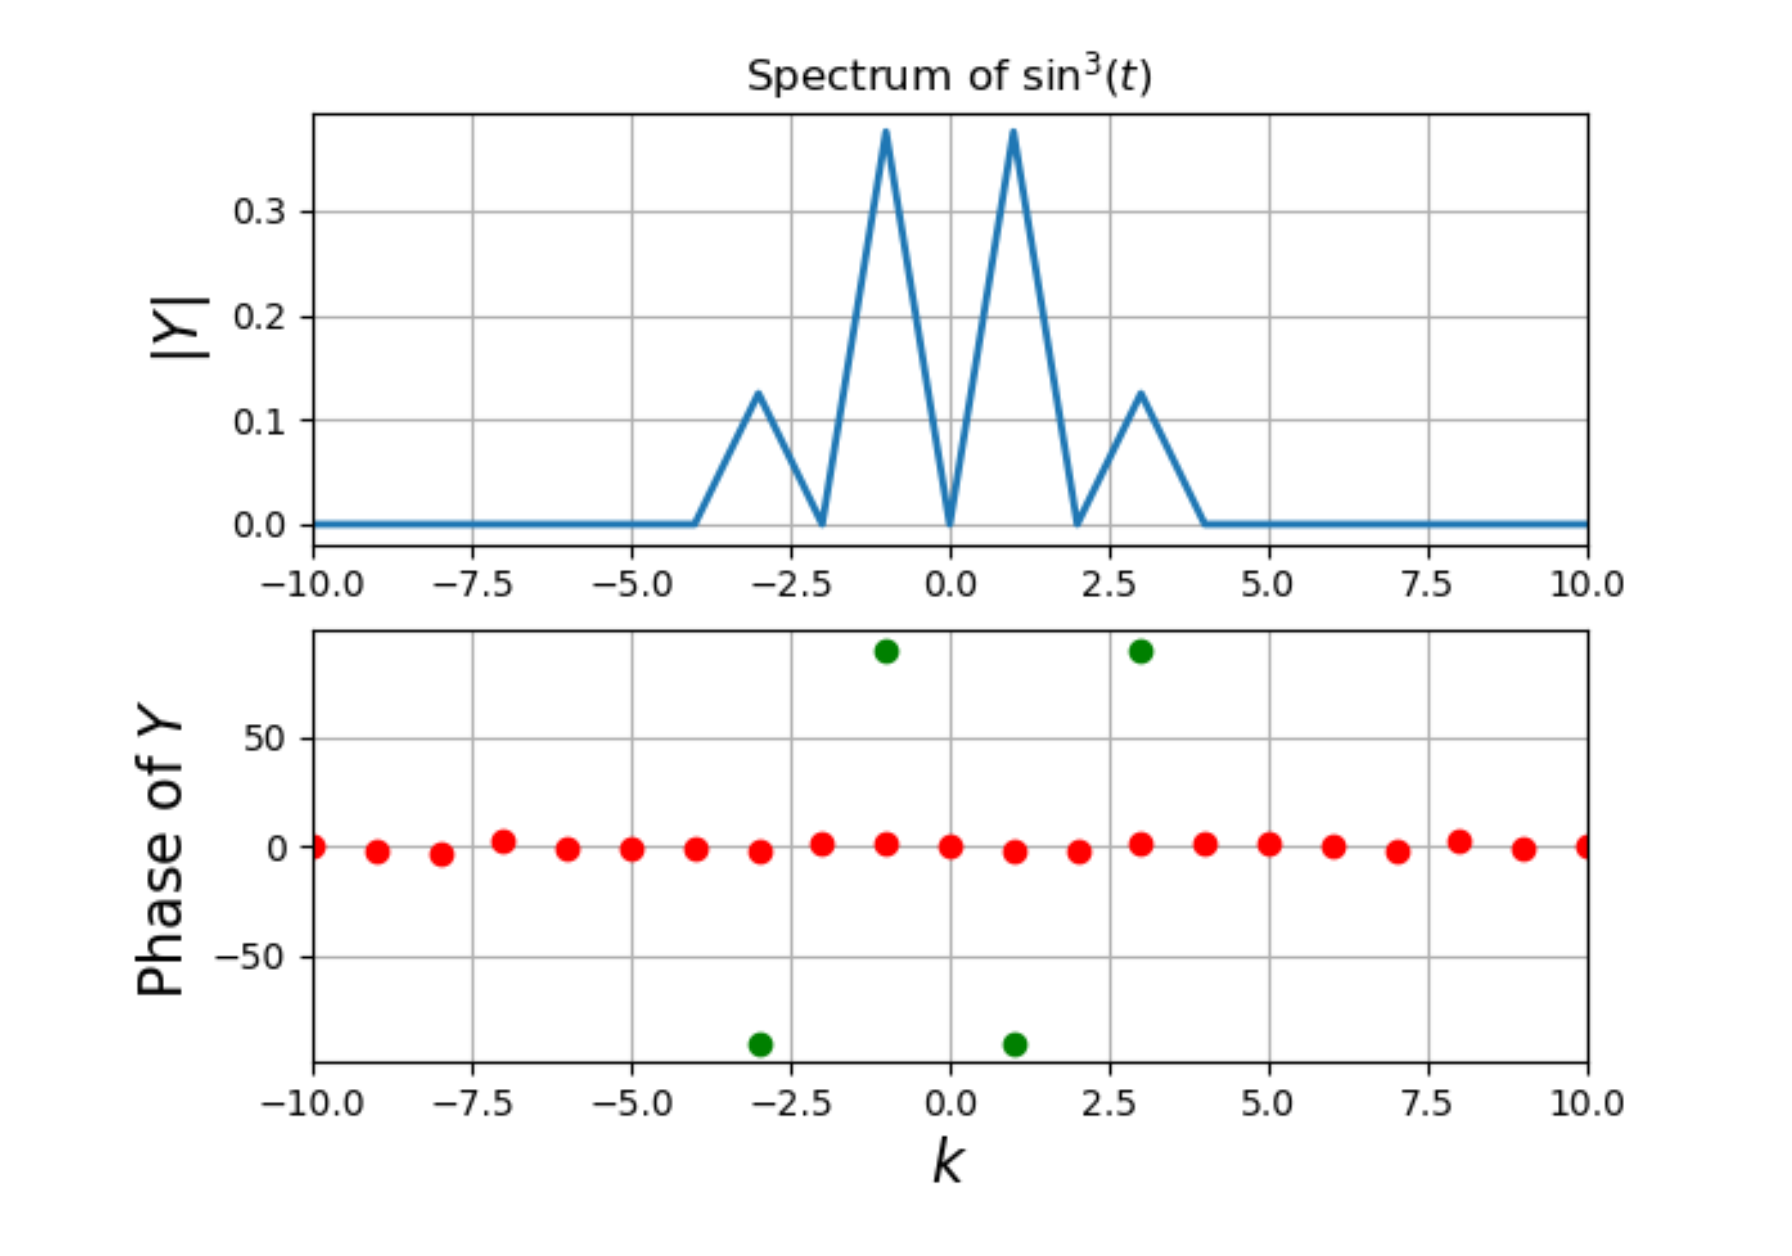
\includegraphics[scale=0.3]{Figure1.png}}\\
We can clearly see that the signal is not sin($\sqrt{2}$t), and so the spectrum of the signal looks as below.\\
{\centering 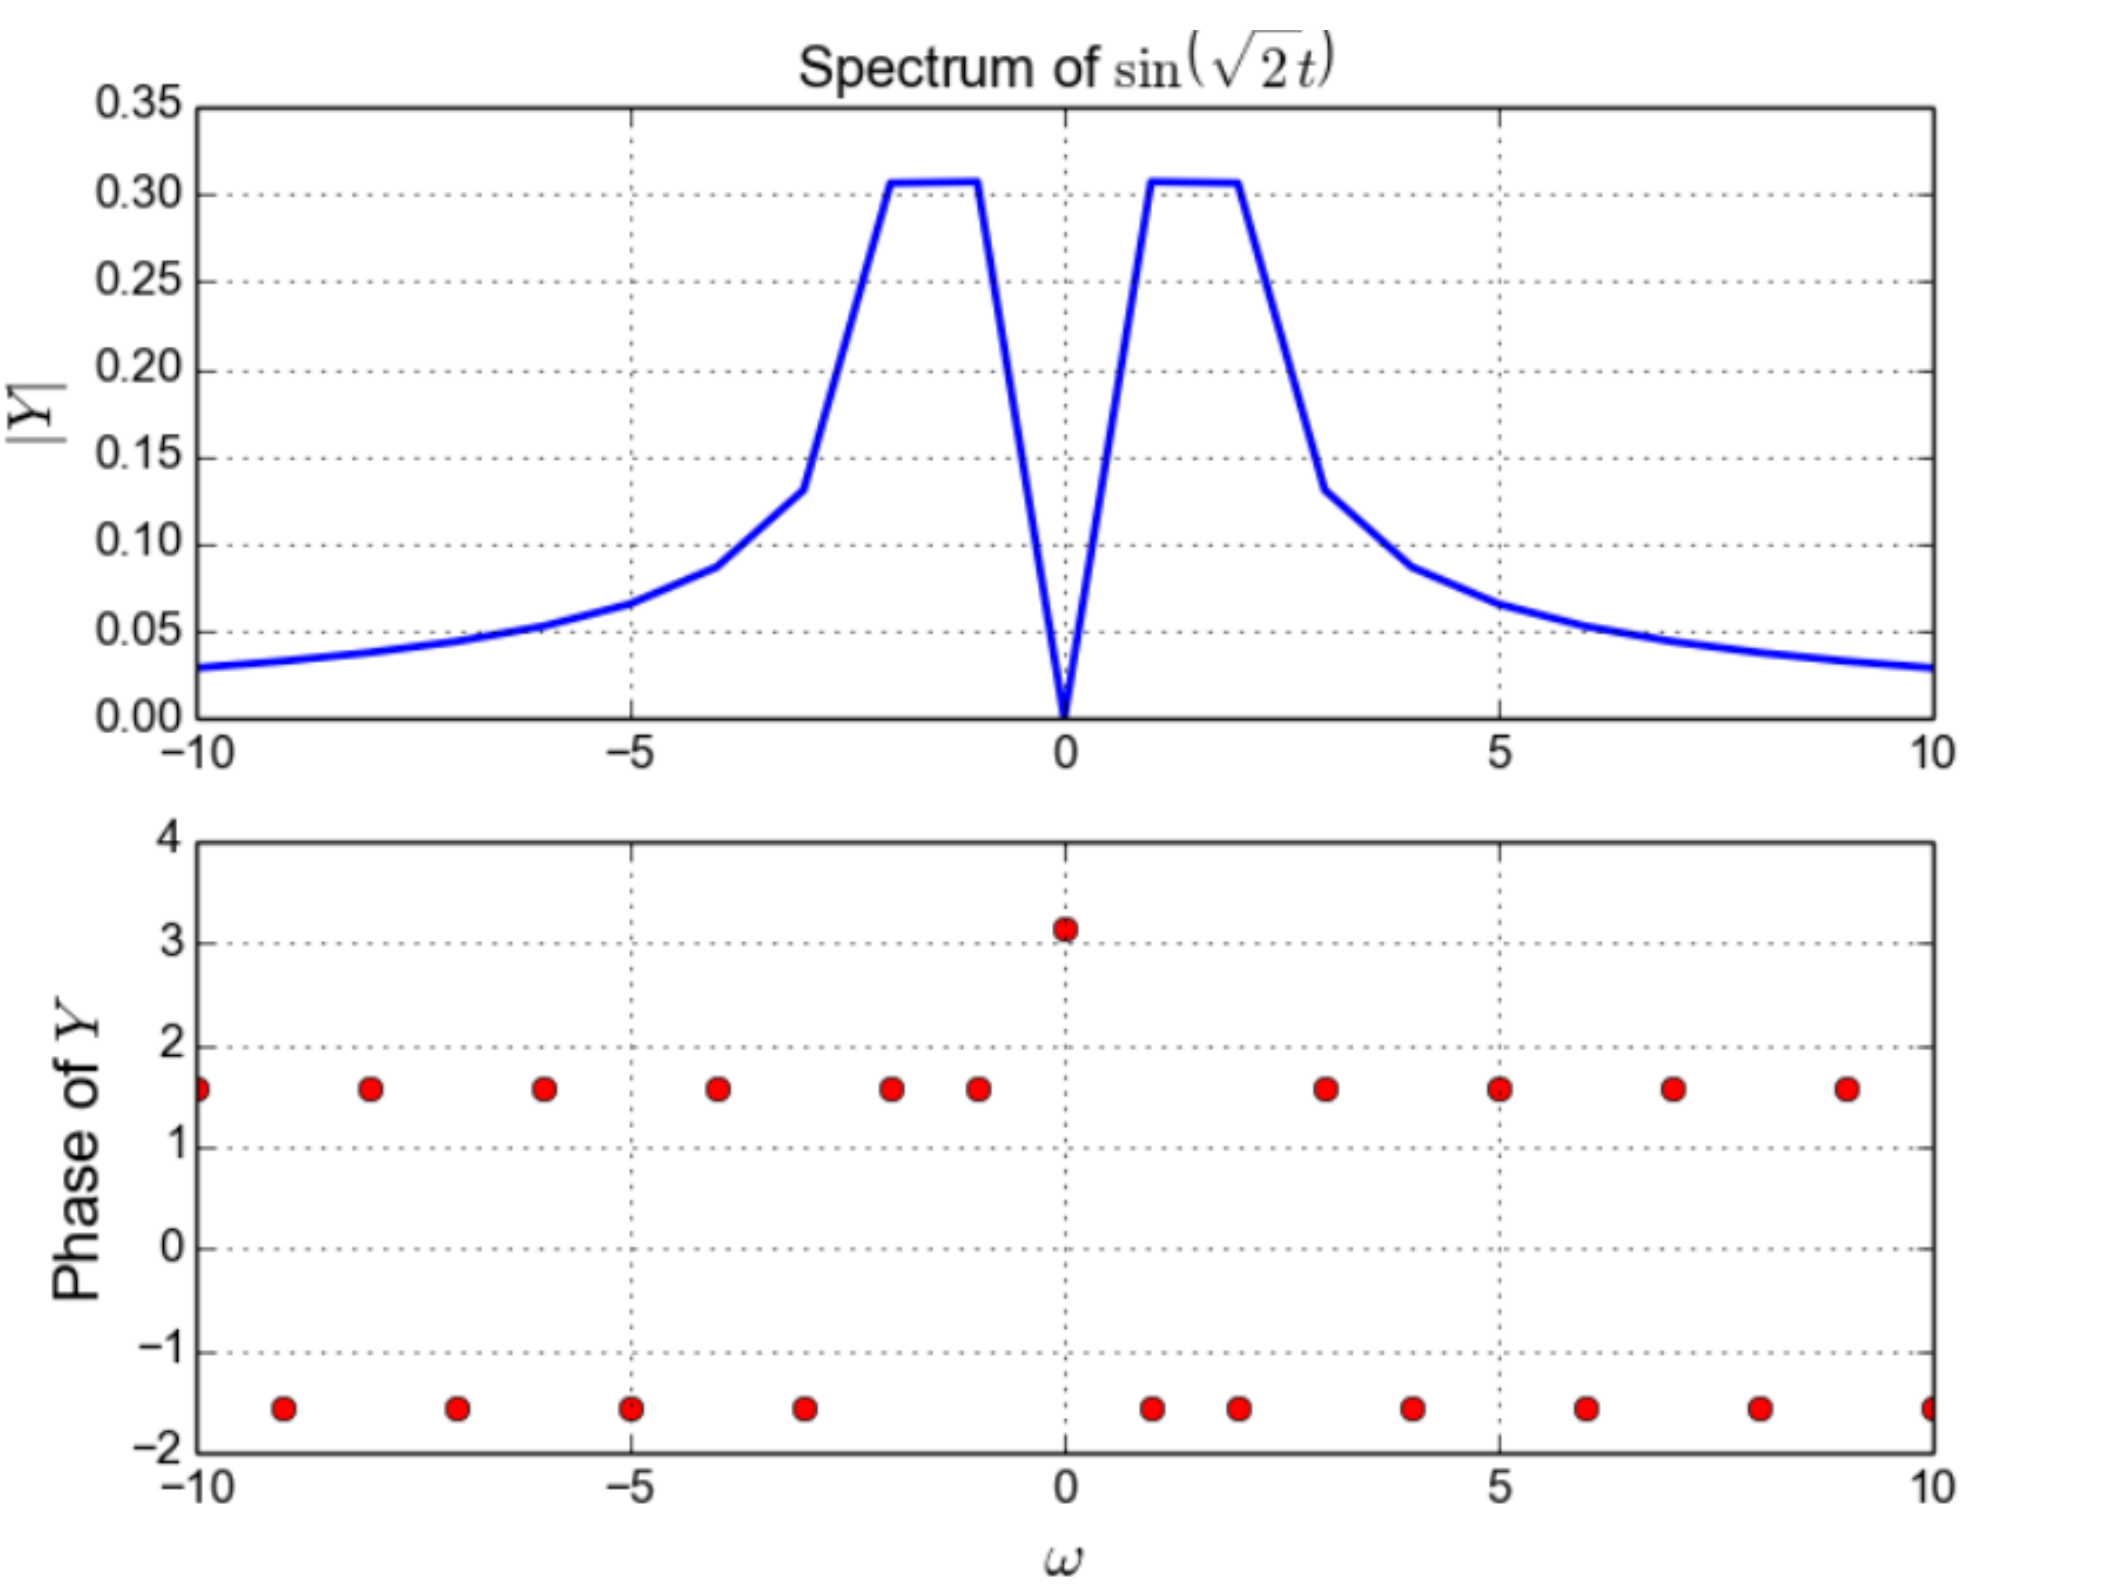
\includegraphics[scale=0.3]{Figure2.png}}\\
\begin{verbatim}
from pylab import * 
t=linspace(-pi,pi,65);t=t[:-1] 
dt=t[1]-t[0];fmax=1/dt
y=sin(sqrt(2)*t)
y[0]=0
y=fftshift(y) # make y start with y(t=0)
Y=fftshift(fft(y))/64.0 
w=linspace(-pi*fmax,pi*fmax,65);w=w[:-1]
figure()
subplot(2,1,1)
plot(w,abs(Y),lw=2)
xlim([-10,10])
ylabel(r"$|Y|$",size=16)
title(r"Spectrum of $\sin\left(\sqrt{2}t\right)$") 
grid(True)
subplot(2,1,2)
plot(w,angle(Y),’ro’,lw=2)
xlim([-10,10])
ylabel(r"Phase of $Y$",size=16)
xlabel(r"$\omega$",size=16)
grid(True)
show()
\end{verbatim}

Due to the jump at $-\pi$ and $\pi$ we do not get two peaks and instead get a maximum which is decaying. Due to this we cannot find the frequency of a periodic but asymmetric signal if we have its spectrum.To make the peaks more visible we window the signal.

\section{Windowing}

If we window the signal by damping the near the end of the function as it jumps we get a signal closer to the original. This is known as a window sequence and the DFT is obtained by convolution both the signals.\\

\begin{center}
$g(n)=f(n)w(n)$\\

$G_{k}=\sum_{n=0}^{N-1} F_{n}W_{k-n}$\\
\end{center}
In this assignment we are going to be using a window called Hamming
Window.\\
i.e.

\begin{equation*}
w[n]=\begin{cases}
0.54 + 0.46cos( 2\pi n/N-i ), & |n|<\frac{N-1}{2}\\
0, & \text{else}
\end{cases}
\end{equation*}
\section{Plot with Windowing}
If we multiply sin($ \sqrt{2}$t) with w[n] we get a windowed signal with damping at the end.\\
{\centering 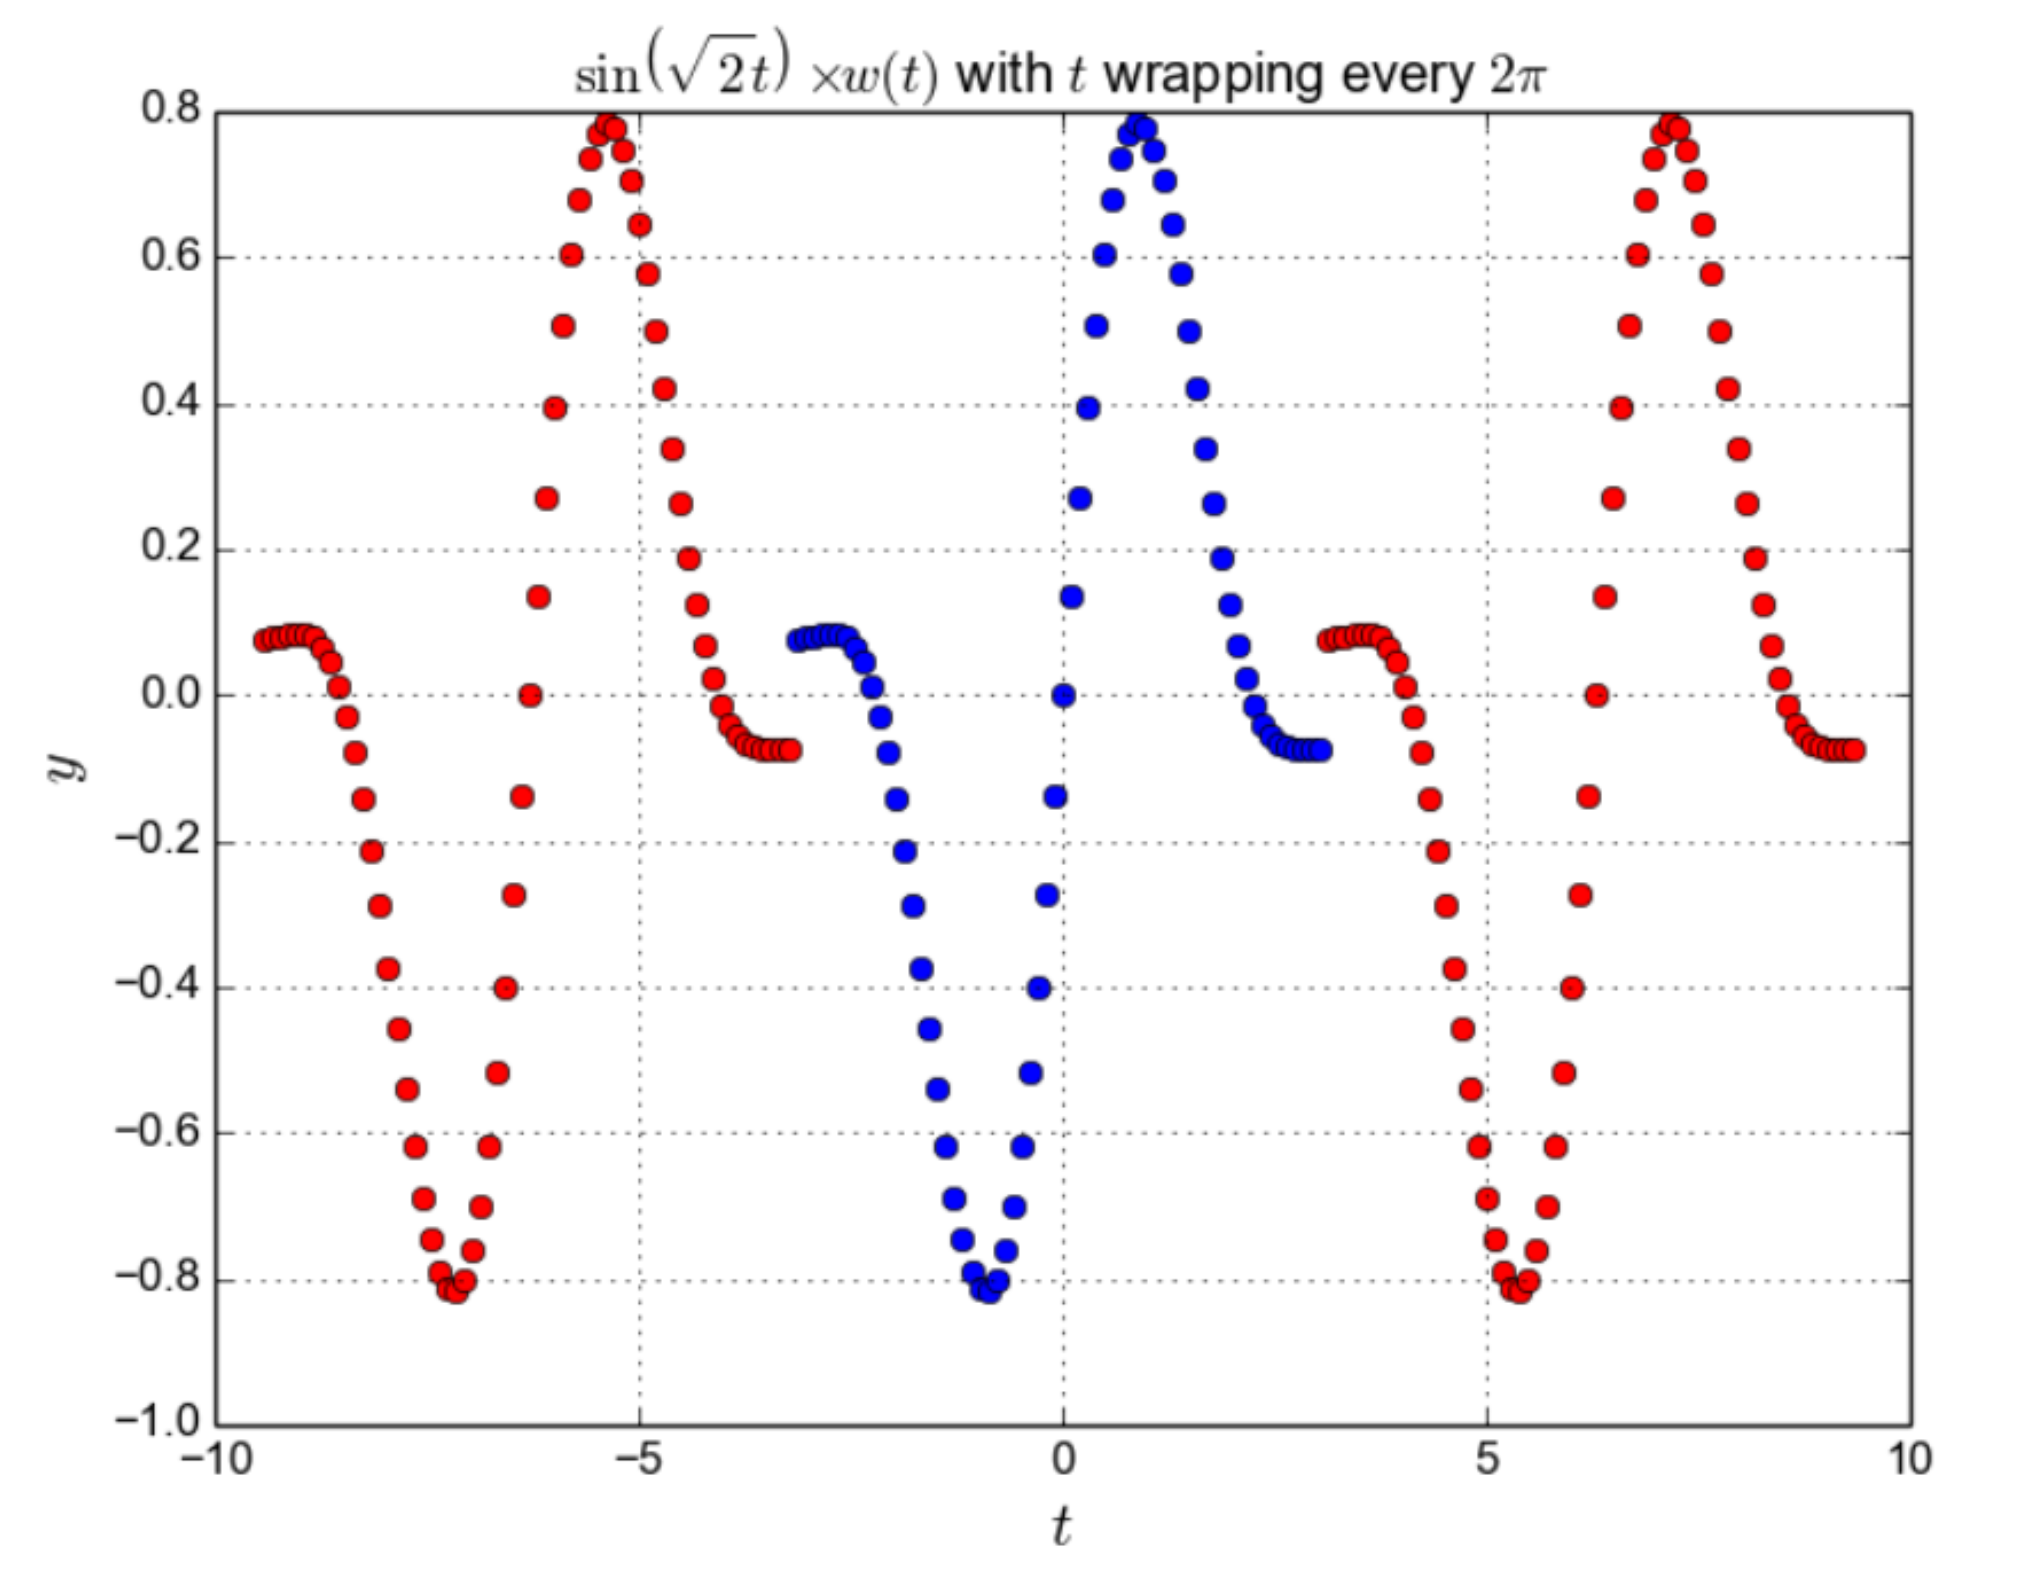
\includegraphics[scale=0.3]{Figure3.png}}\\
If we obtain DFT of the signal with previous procedure we get a better spectrum. If we increase the sampling then we get a much better plot with defined peaks.\\
{\centering 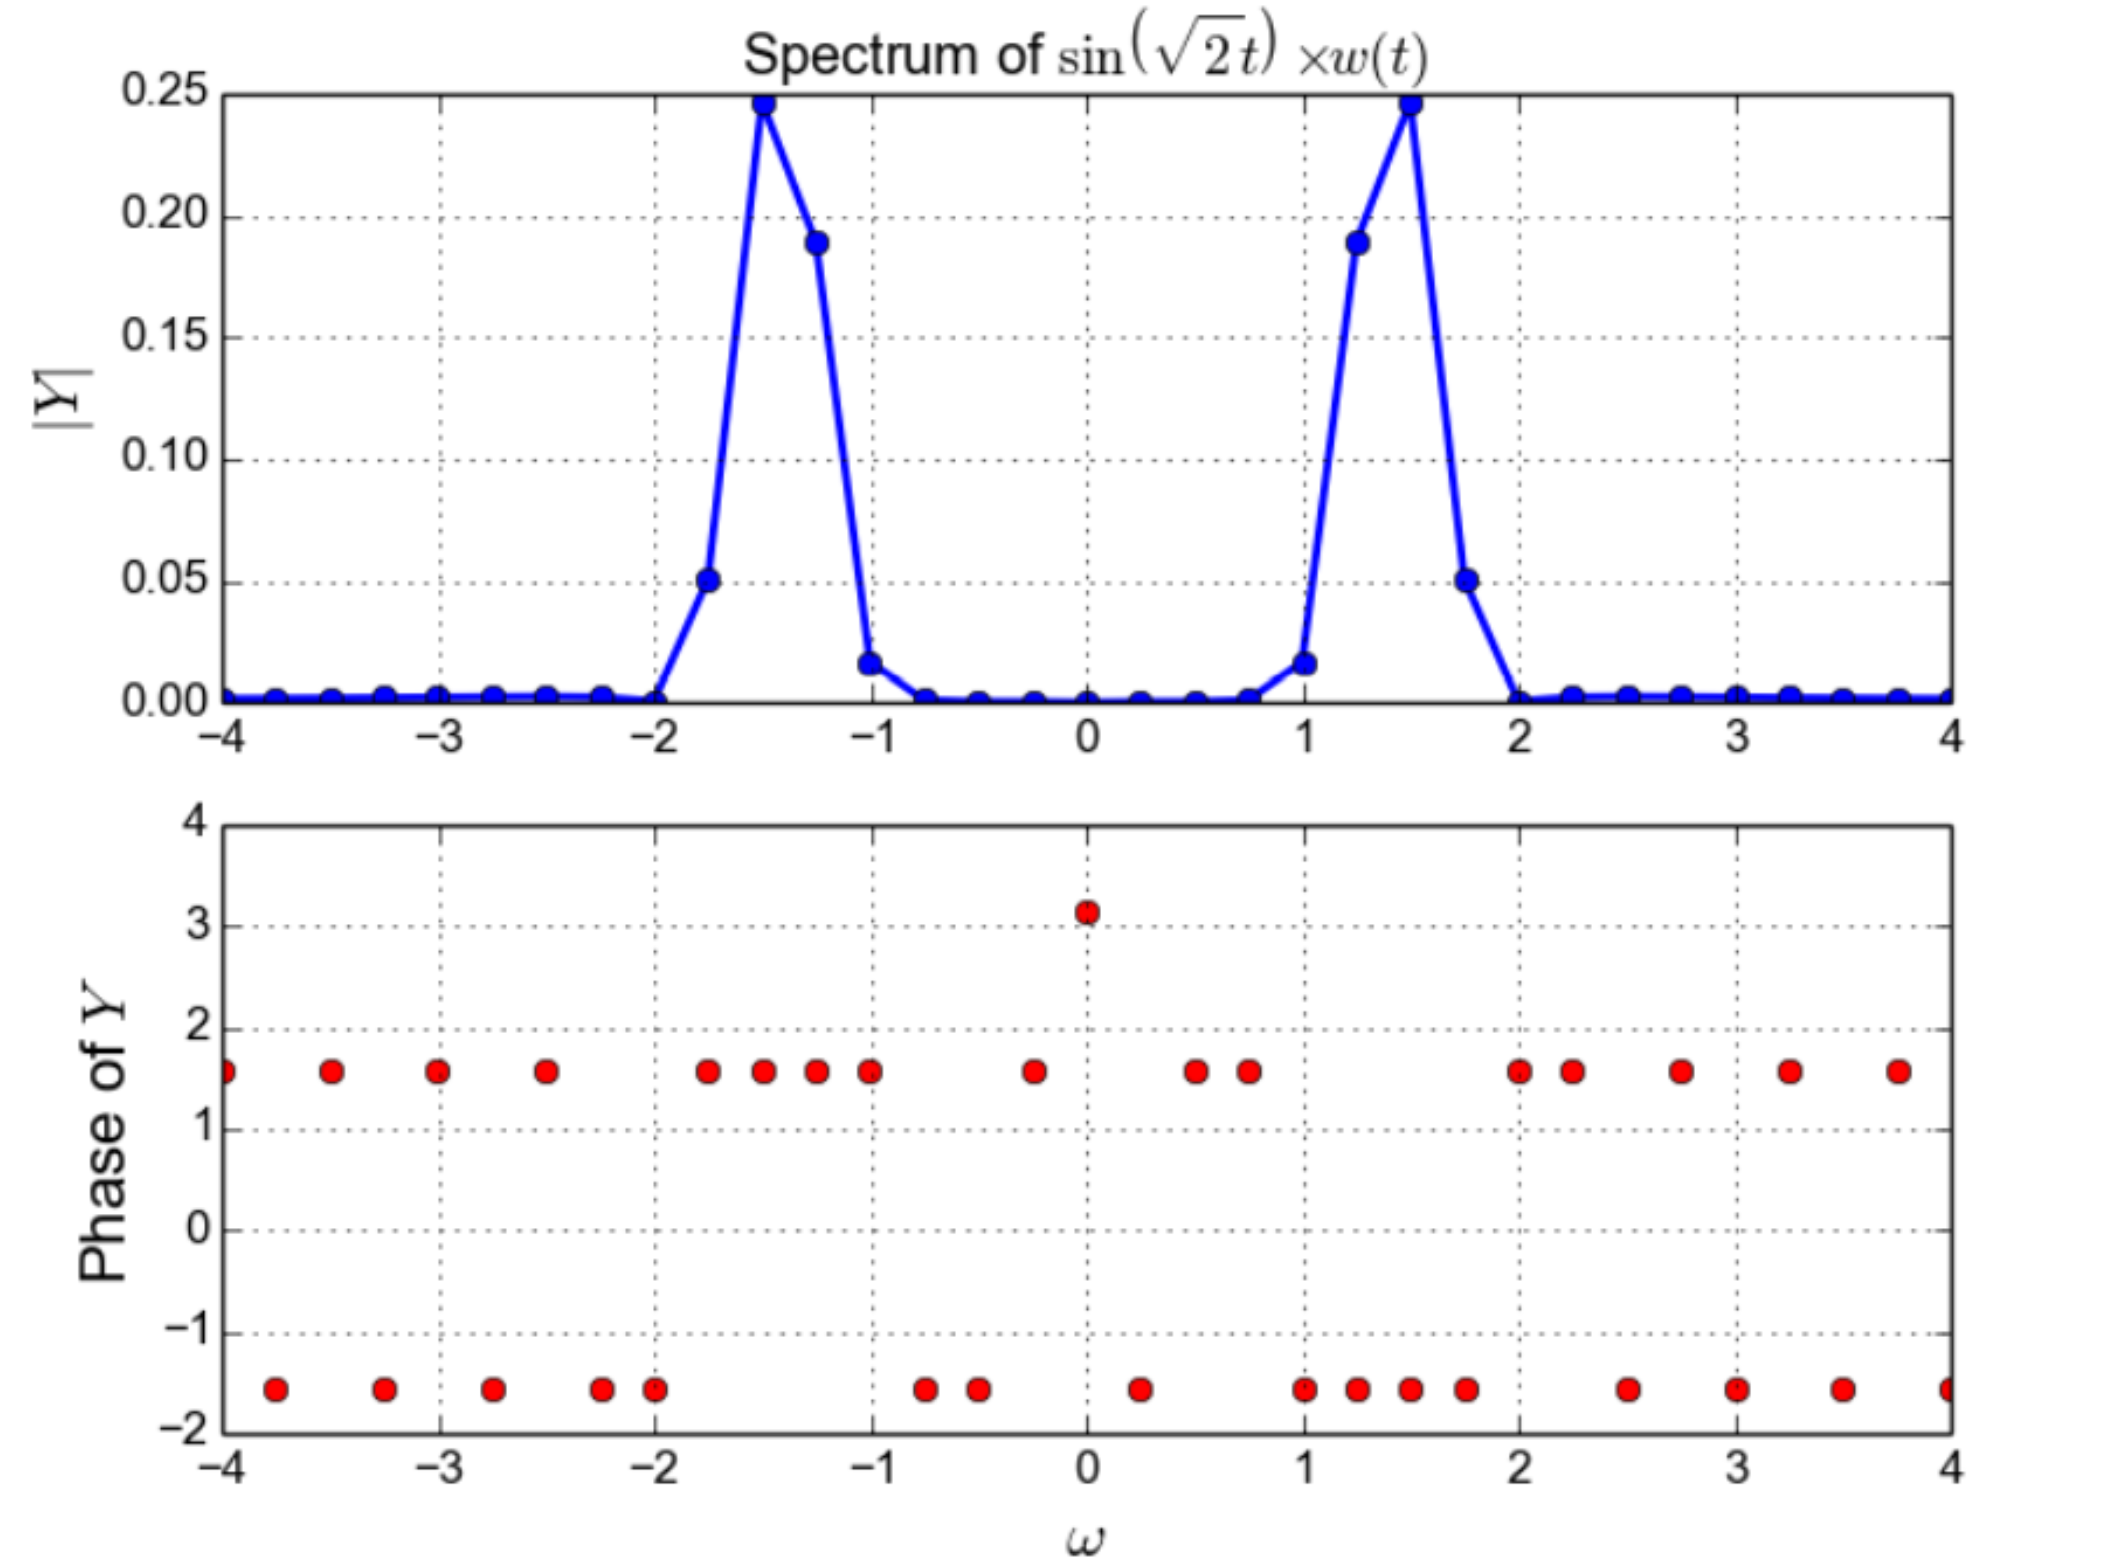
\includegraphics[scale=0.3]{Figure4.png}}\\


\chapter{The Assignment}

\section{Problem 1}
In the first problem we have to find the frequency spectrum of $cos^{3}(0.86t)$. Similar to previous assignment we first sample the signal. We then find the DFT of the signal and and plot it against frequency. In this assignment we additionally multiply a window with same amount of samples and then find the DFT.\\
We first find the spectrum of the signal without windowing.\\
\begin{verbatim}
N=2**8 
w_0=0.86
t=linspace(-4*pi,4*pi,N+1);t=t[:-1] 
dt=t[1]-t[0];fmax=1/dt
n=arange(N) 
wnd=fftshift(0.54+0.46*cos(2*pi*n/(N-1)))
y=cos(w_0*t)**3
y[0]=0
Y=fftshift(fft(y))/N 
w=linspace(-pi*fmax,pi*fmax,N+1);w=w[:-1]
figure()
subplot(2,1,1)
plot(w,abs(Y),’bo-’)
xlim([-5,5])
ylabel(r"$|Y|$",size=16)
title(r"Spectrum of $cos^3(W_0t)$") 
subplot(2,1,2)
plot(w,angle(Y),’ro’)
xlim([-4,4])
ylabel(r"Phase of $Y$",size=16) 
xlabel(r"$\omega$",size=16)
\end{verbatim}
{\centering 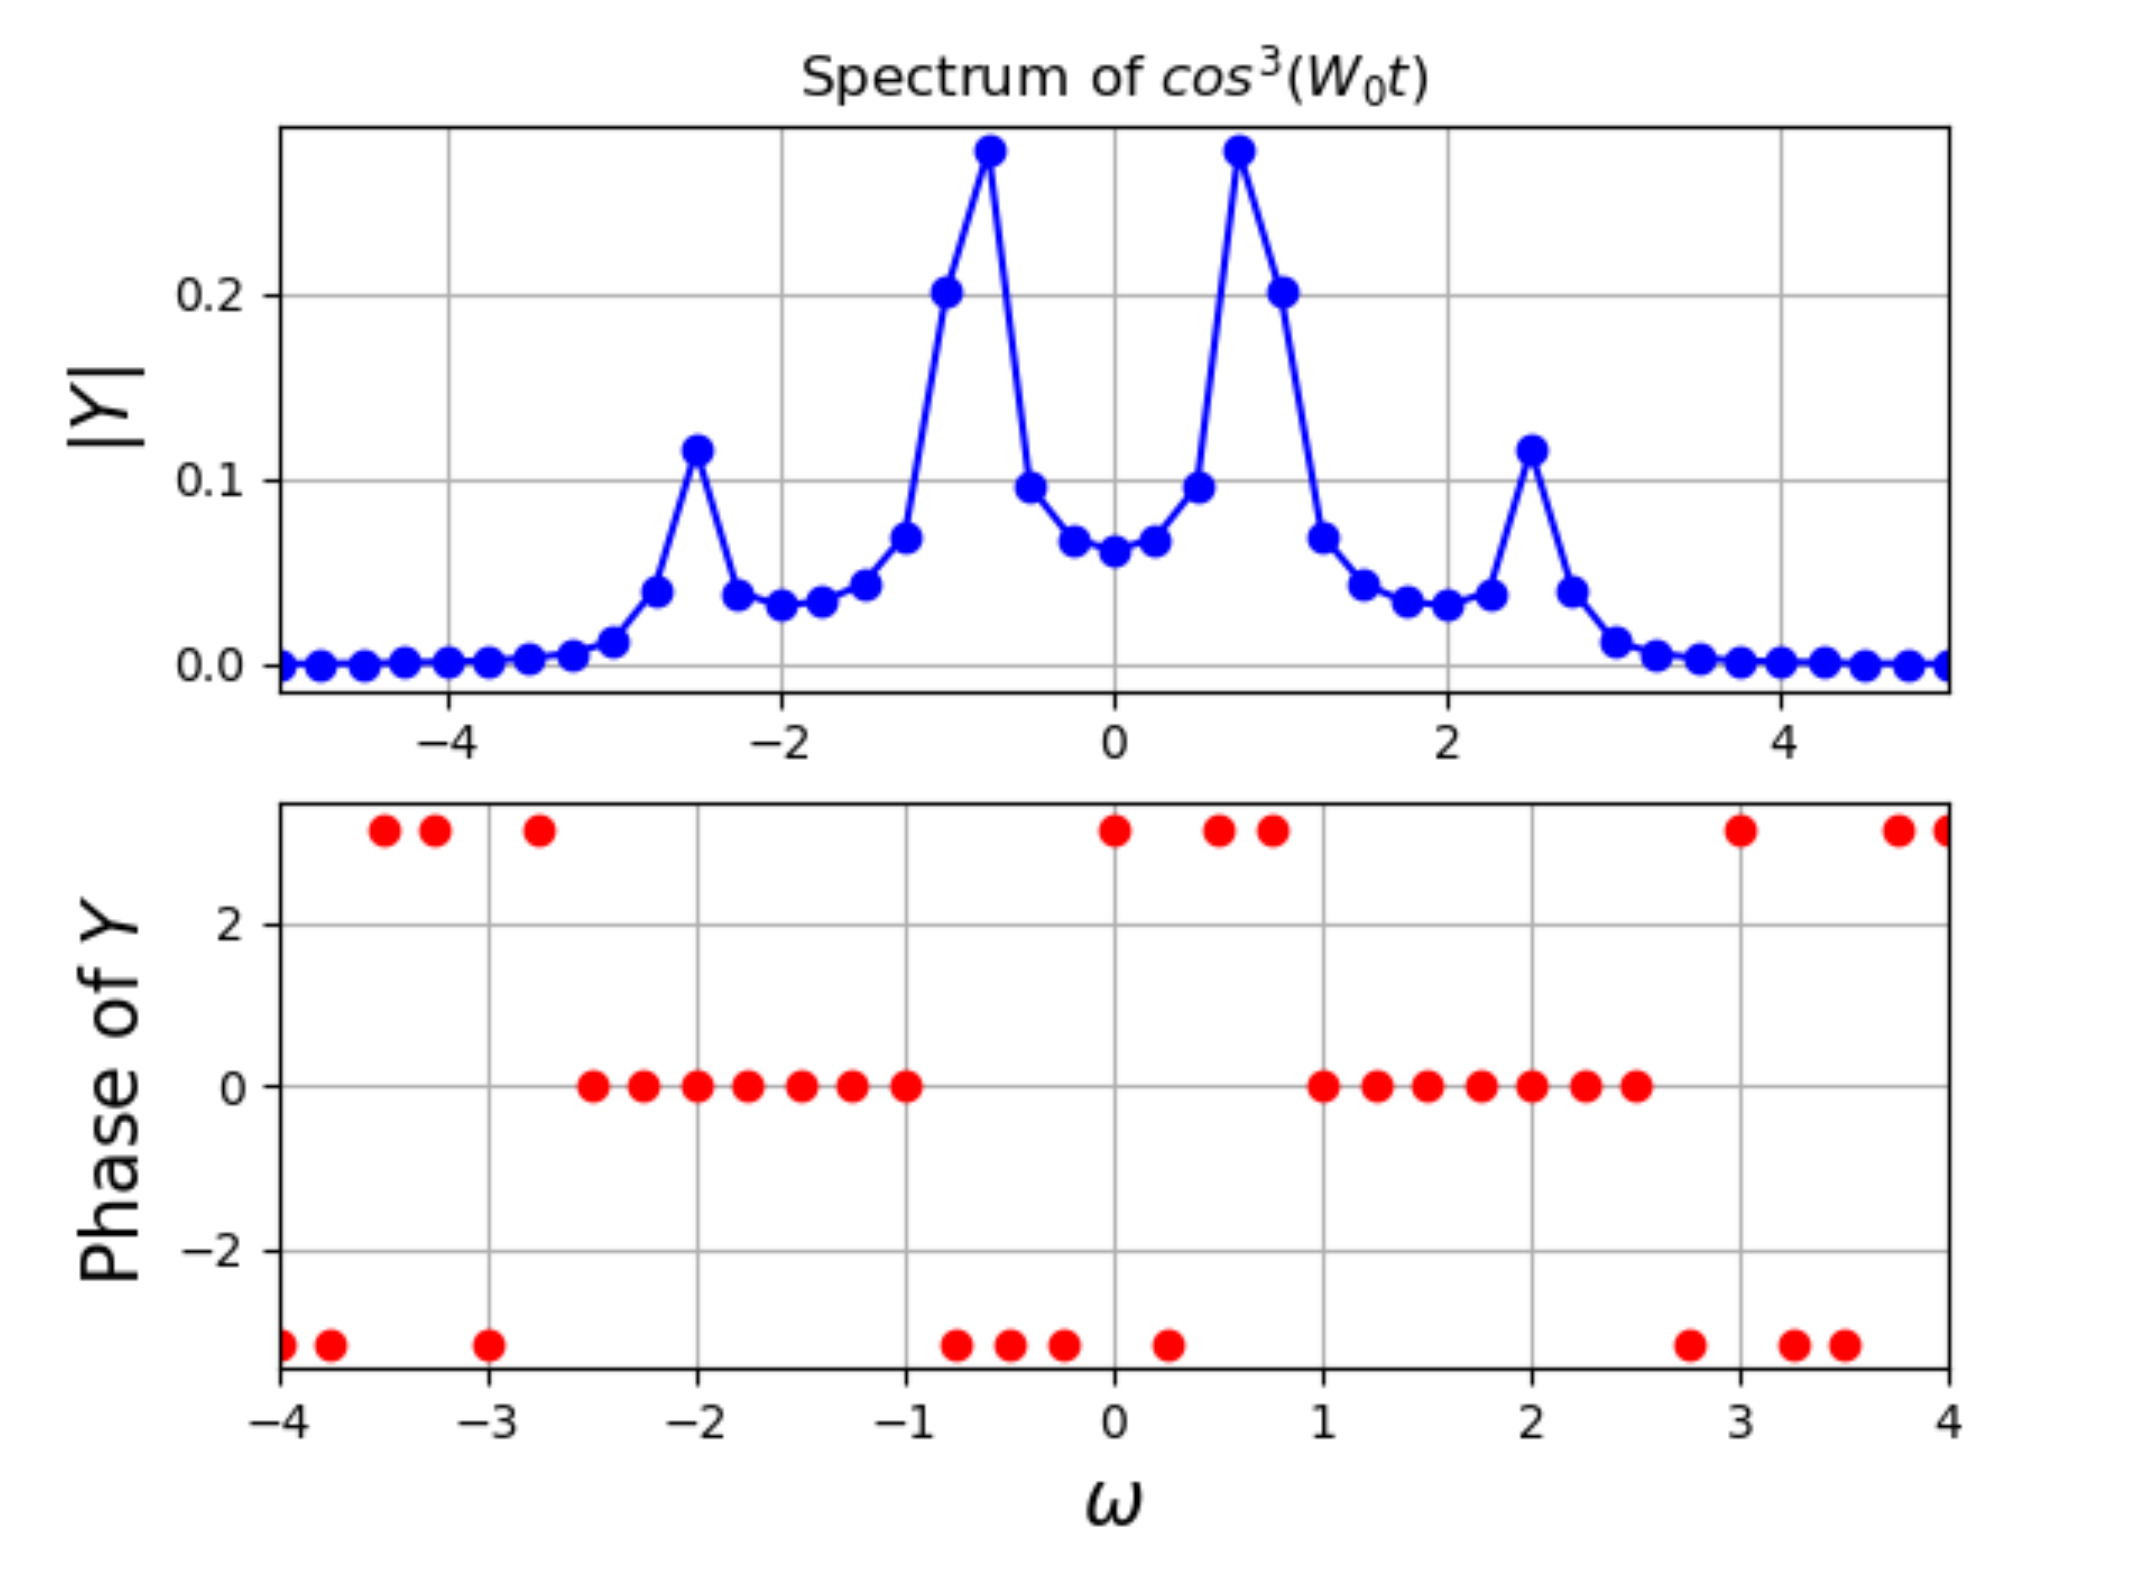
\includegraphics[scale=0.3]{Figure5.png}}\\
Now we obtain the spectrum after windowing.

\begin{verbatim}
y=(cos(w_0*t)**3)*wnd 
y[0]=0
y=fftshift(y) 
Y=fftshift(fft(y))/N
w=linspace(-pi*fmax,pi*fmax,N+1);w=w[:-1] 
figure()
subplot(2,1,1)
plot(w,abs(Y),’bo-’)
xlim([-5,5])
ylabel(r"$|Y|$",size=16) 
title(r"Spectrum of $cos(W_0t)*w(t)$") 
subplot(2,1,2)
plot(w,angle(Y),’ro’)
xlim([-5,5])
ylabel(r"Phase of $Y$",size=16)
xlabel(r"$\omega$",size=16)
\end{verbatim}
{\centering 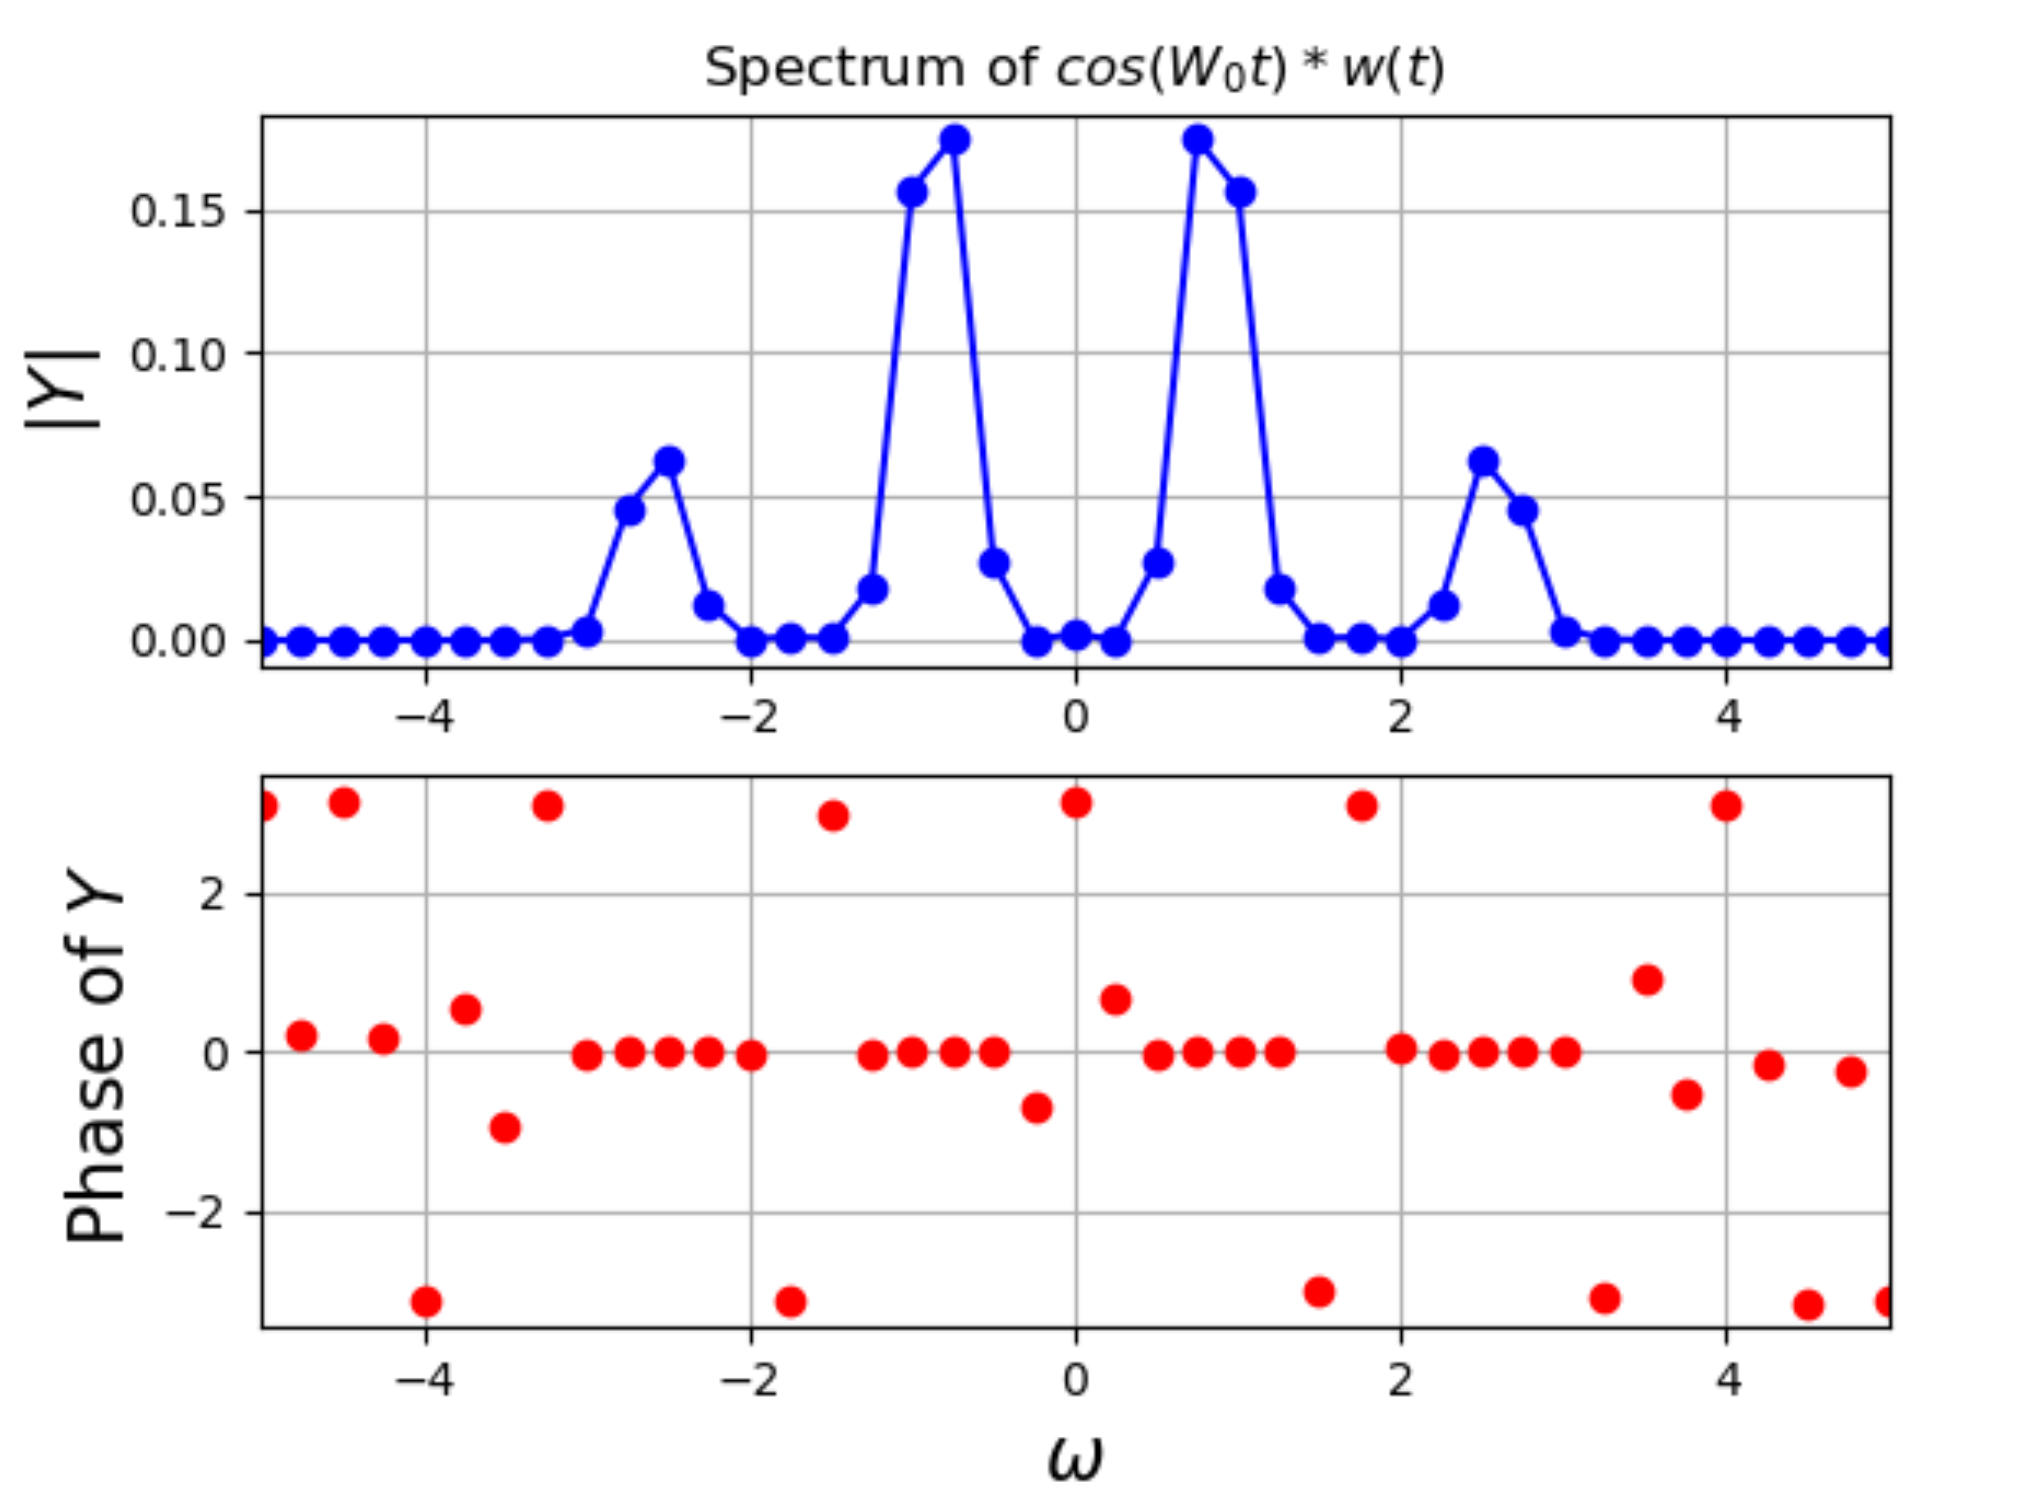
\includegraphics[scale=0.3]{Figure6.png}}\\

We obtain much better peaks in the spectrum when we window the signal.




\section{Problem 2}

In this problem we have a 128 element vector of the form $cos(w_{0}t+\delta)$. Here $w_{0}$ lies between 0.5 and 1.5 and $\delta$ is arbitrary. We will take an arbitrary $w_{0}$ and $\delta$ and try to predict the values from its spectrum.\\

\begin{verbatim}

w0=0.84
delta=0.9
N=128
n=arange(N) 
wnd_2=fftshift(0.54+0.46*cos(2*pi*n/N-1))
t=linspace(-pi,pi,N+1);t=t[:-1] 
dt=t[1]-t[0];fmax=1/dt 
w=linspace(-pi*fmax,pi*fmax,N+1);w=w[:-1] 
y_2=cos(w0*t+delta)*wnd_2
y_2[0]=0
figure()
plot(t,y_2)
Y_2=fftshift(fft(y_2)/N) 
figure()
subplot(2,1,1)
xlim([-4,4])
plot(w,abs(Y_2))
subplot(2,1,2)
xlim([-4,4])
plot(w,angle(Y_2),’ro’)
w_2p = sum(abs(Y_2**1.7*w))/sum(abs(Y_2)**1.7) 
del_p=angle(Y_2[::-1][argmax(abs(Y_2[::-1]))]) 
if del_p>=0:
  del_p=pi-del_p 
else:
  del_p=pi+del_p
print(’Actual Values : W={} Delta={}’.format(w0,delta)) 
print(’Predicted Values:W= {}Delta={}’.format(w_2p,del_p))
\end{verbatim}
We estimate $\omega_{0}$ by finding estimation of spectrum.\\
\begin{equation*}
\omega_{0}=\frac{\sum(Yw)^{p}}{\sum (w)}
\end{equation*}

On trying different values of p, for p = 1.7 we found the best estimate of $\omega_{0}$.
For estimating phase we can just find the angle of spectrum at peak value of the magnitude since the phase doesn’t change much.


\section{Problem 3}
In this problem we have to find the values of $w_{0}$ and $\delta$ but with noise. Noise can be generated using \textbf{\textit{0.1rand(128)}} with max amplitude of 0.1 and of 128 samples.\\

\begin{verbatim}
y_3=y_2+0.1*randn(N)
Y_3=fftshift(fft(y_3)/N)
w_2p = sum(abs(Y_3**2.4*w))/sum(abs(Y_3)**2.4)
del_p=angle(Y_2[argmax(abs(Y_3))])
if del_p>=0:
	del_p=pi-del_p
else: del_p=pi+del_p
\end{verbatim}


Similar to previous problem we estimate $w_{0}$. But in this case the coefficients p = 2.4 for obtaining better estimates. Similarly phase closely corresponds to peak value of magnitude.

\section{Problem 4}
In this problem we have to find DFT of\\
\begin{equation*}
cos(16(1.5 + t/2\pi )t)
\end{equation*}
We have to sample from $-\pi$ to $\pi$ in 1024 steps. This is known as a “chirped” signal, and its frequency continuously changes from 16 to 32 radians per second.\\
{\centering 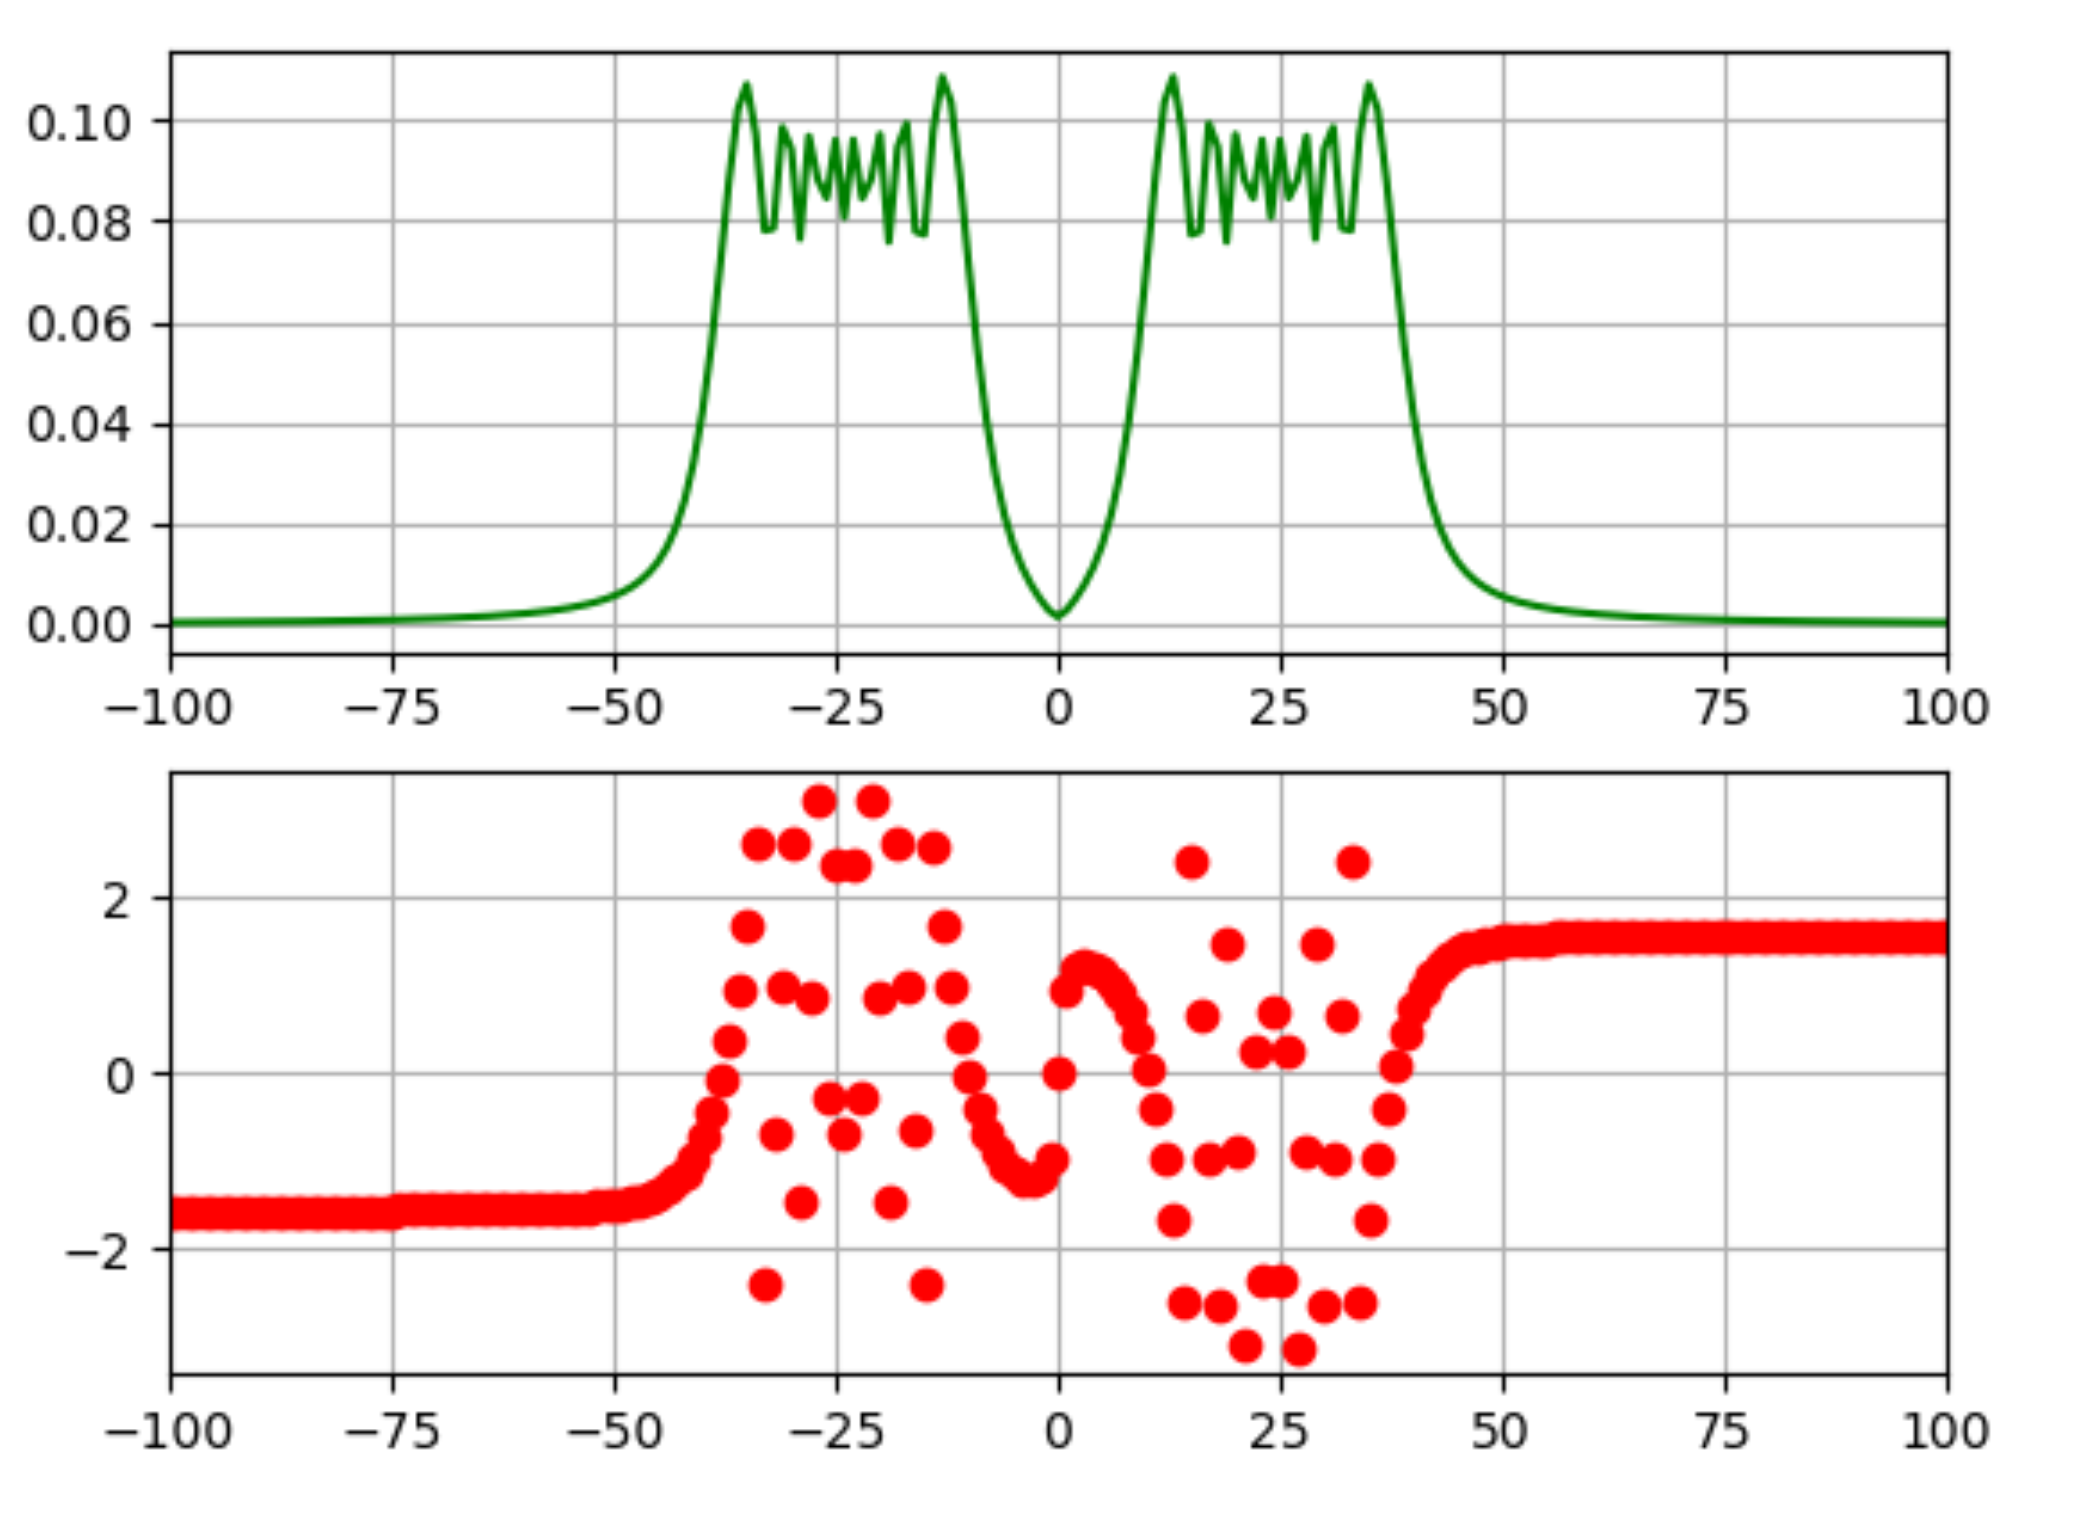
\includegraphics[scale=0.3]{Figure7.png}}\\
\begin{verbatim}
N=2**10
t=linspace(-pi,pi,N+1);t=t[:-1]
dt=t[1]-t[0];fmax=1/dt 
y_4=cos(16*t*(1.5+t/(2*pi)))
Y_4=fftshift(fft(y_4))/N 
w=linspace(-pi*fmax,pi*fmax,N+1);w=w[:-1] 
figure()
subplot(2,1,1) 
plot(w,abs(Y_4),color=’green’) 
xlim([-100,100])
subplot(2,1,2) 
plot(w,angle(Y_4),’ro’)
\end{verbatim}

\section{Problem 5}
In the last problem we have to break the 1024 vector into pieces that are 64 samples wide. Extract the DFT of each and store as a column in a 2D array. Then we have to plot the array as a surface plot to show how the frequency of the signal varies with time.\\
\begin{verbatim}

Y=[]
for i in range(16):
  tlim_1= -pi + 2*pi*i/16
  tlim_2= -pi + 2*pi*(i+1)/16 
  t=linspace(tlim_1,tlim_2,65);t=t[:-1] 
  y=cos(16*t*(1.5+t/(2*pi)))
  y[0]=0 
  Y.append((fftshift(fft(y))/64))
  
Yd=array(Y)
t1=linspace(-pi,pi,16) 
w=linspace(-pi*fmax/2,pi*fmax/2,65);w=w[:-1] 
t1 , w= meshgrid(t1,w)
ax= Axes3D(figure())
surf = ax.plot_surface(t1,w,abs(Yd).T, 
rstride=1, cstride=1, cmap=’viridis’) 
xlabel(’t’)
ylabel(’w’)
\end{verbatim}

We first find DFT for different time intervals in lengths of 64 and 16 sets.Now we form a mesh-grid of t,w and plot DFT of the signal on Z-axis.\\
{\centering 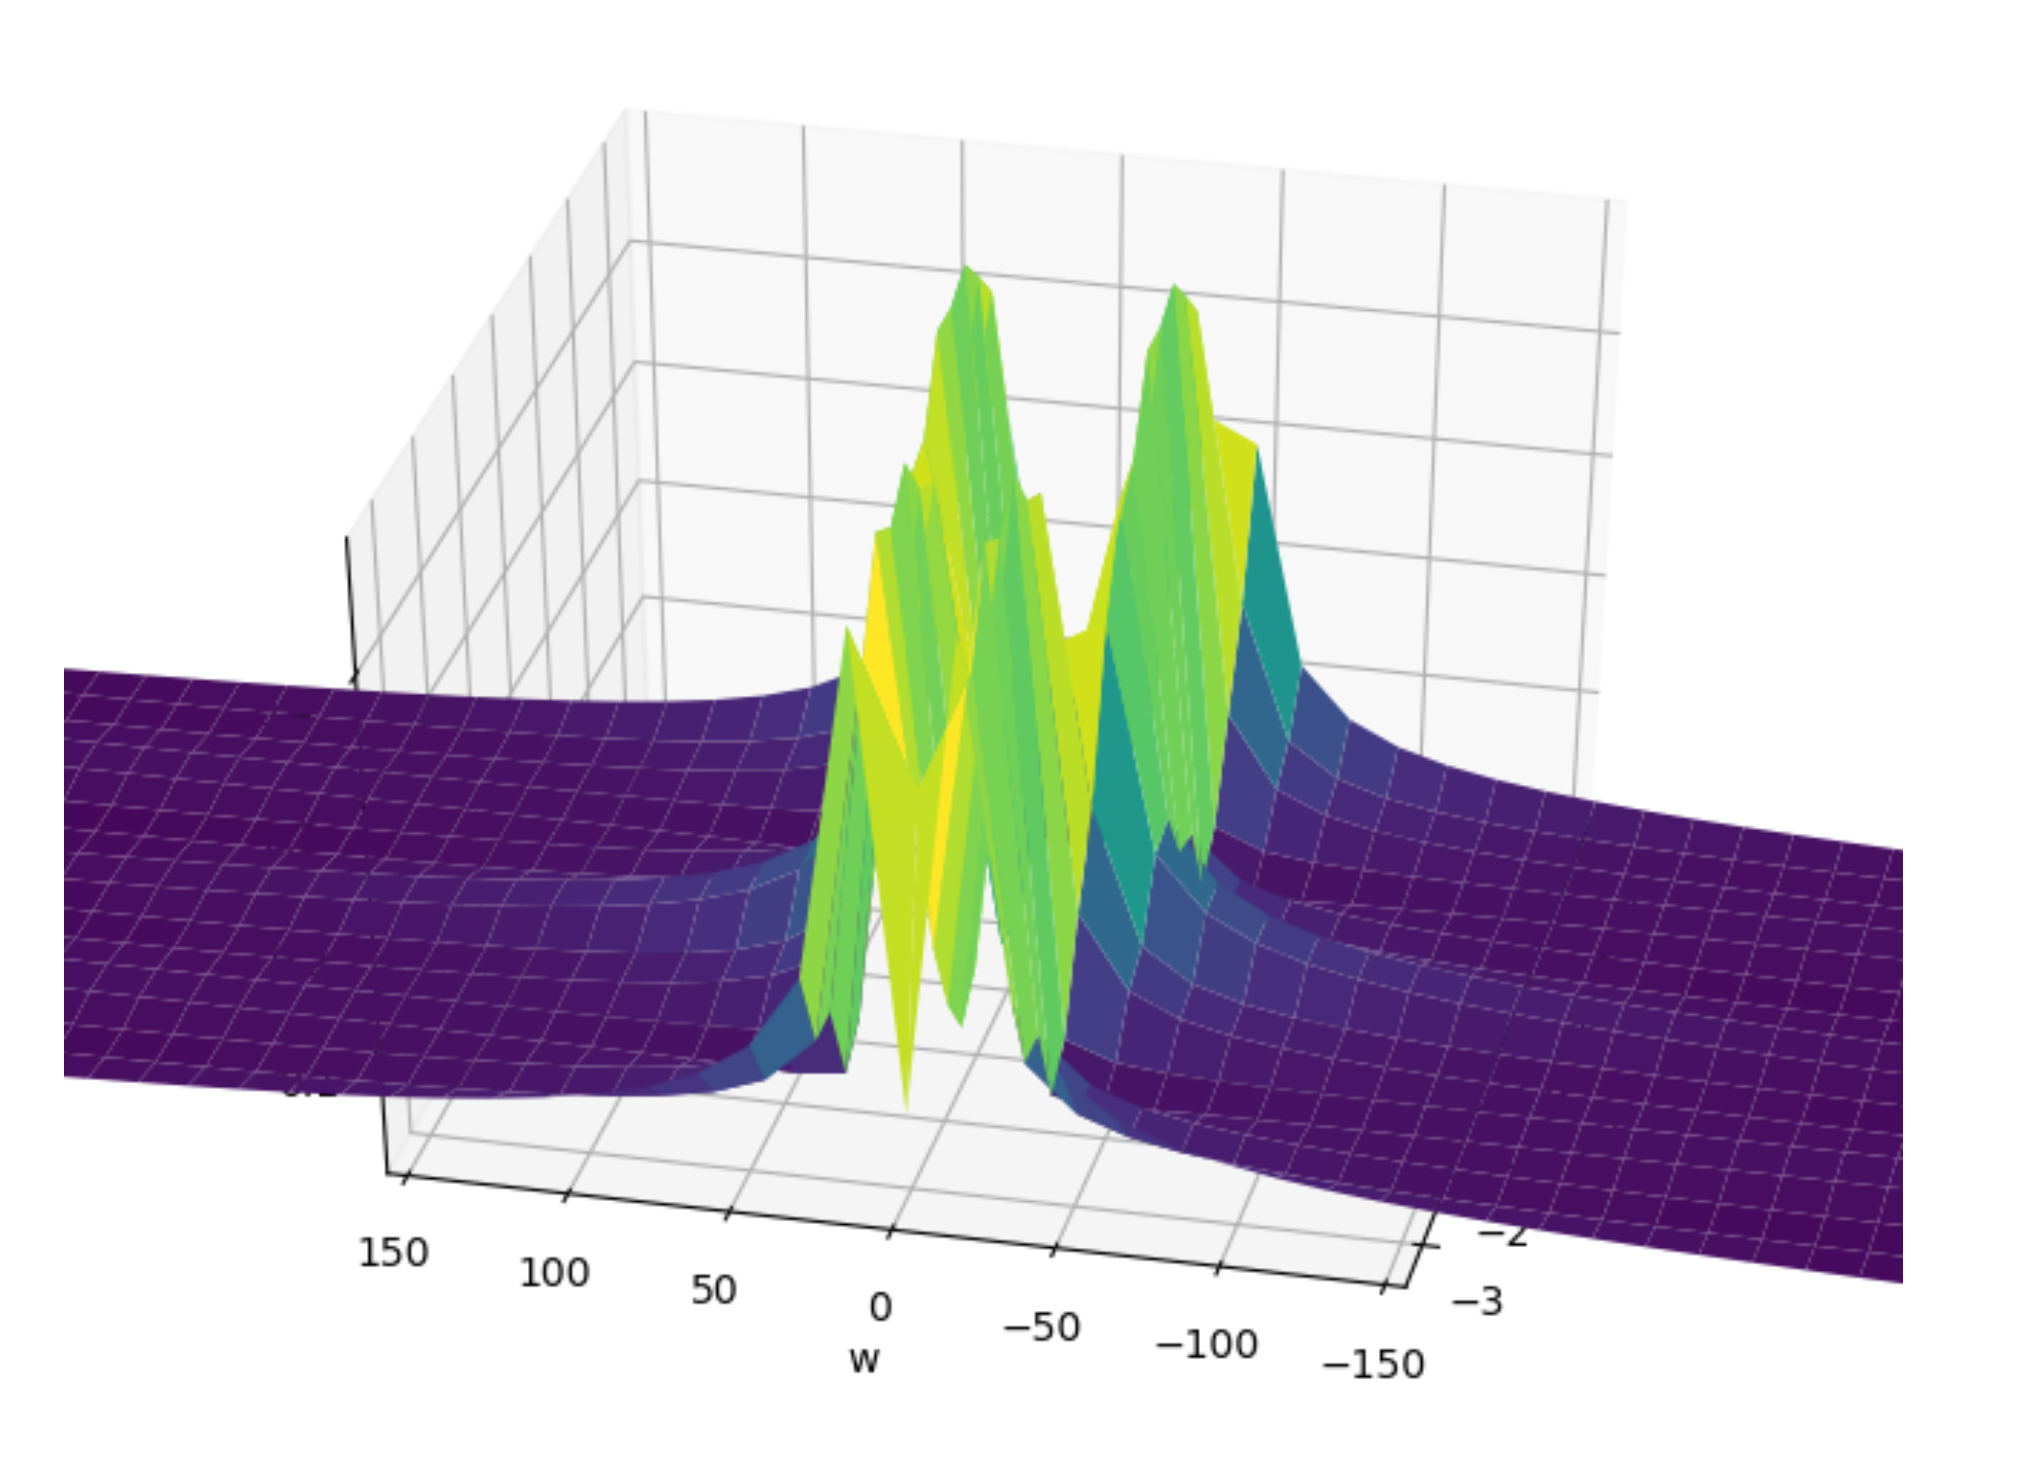
\includegraphics[scale=0.3]{Figure8.png}}\\
{\centering 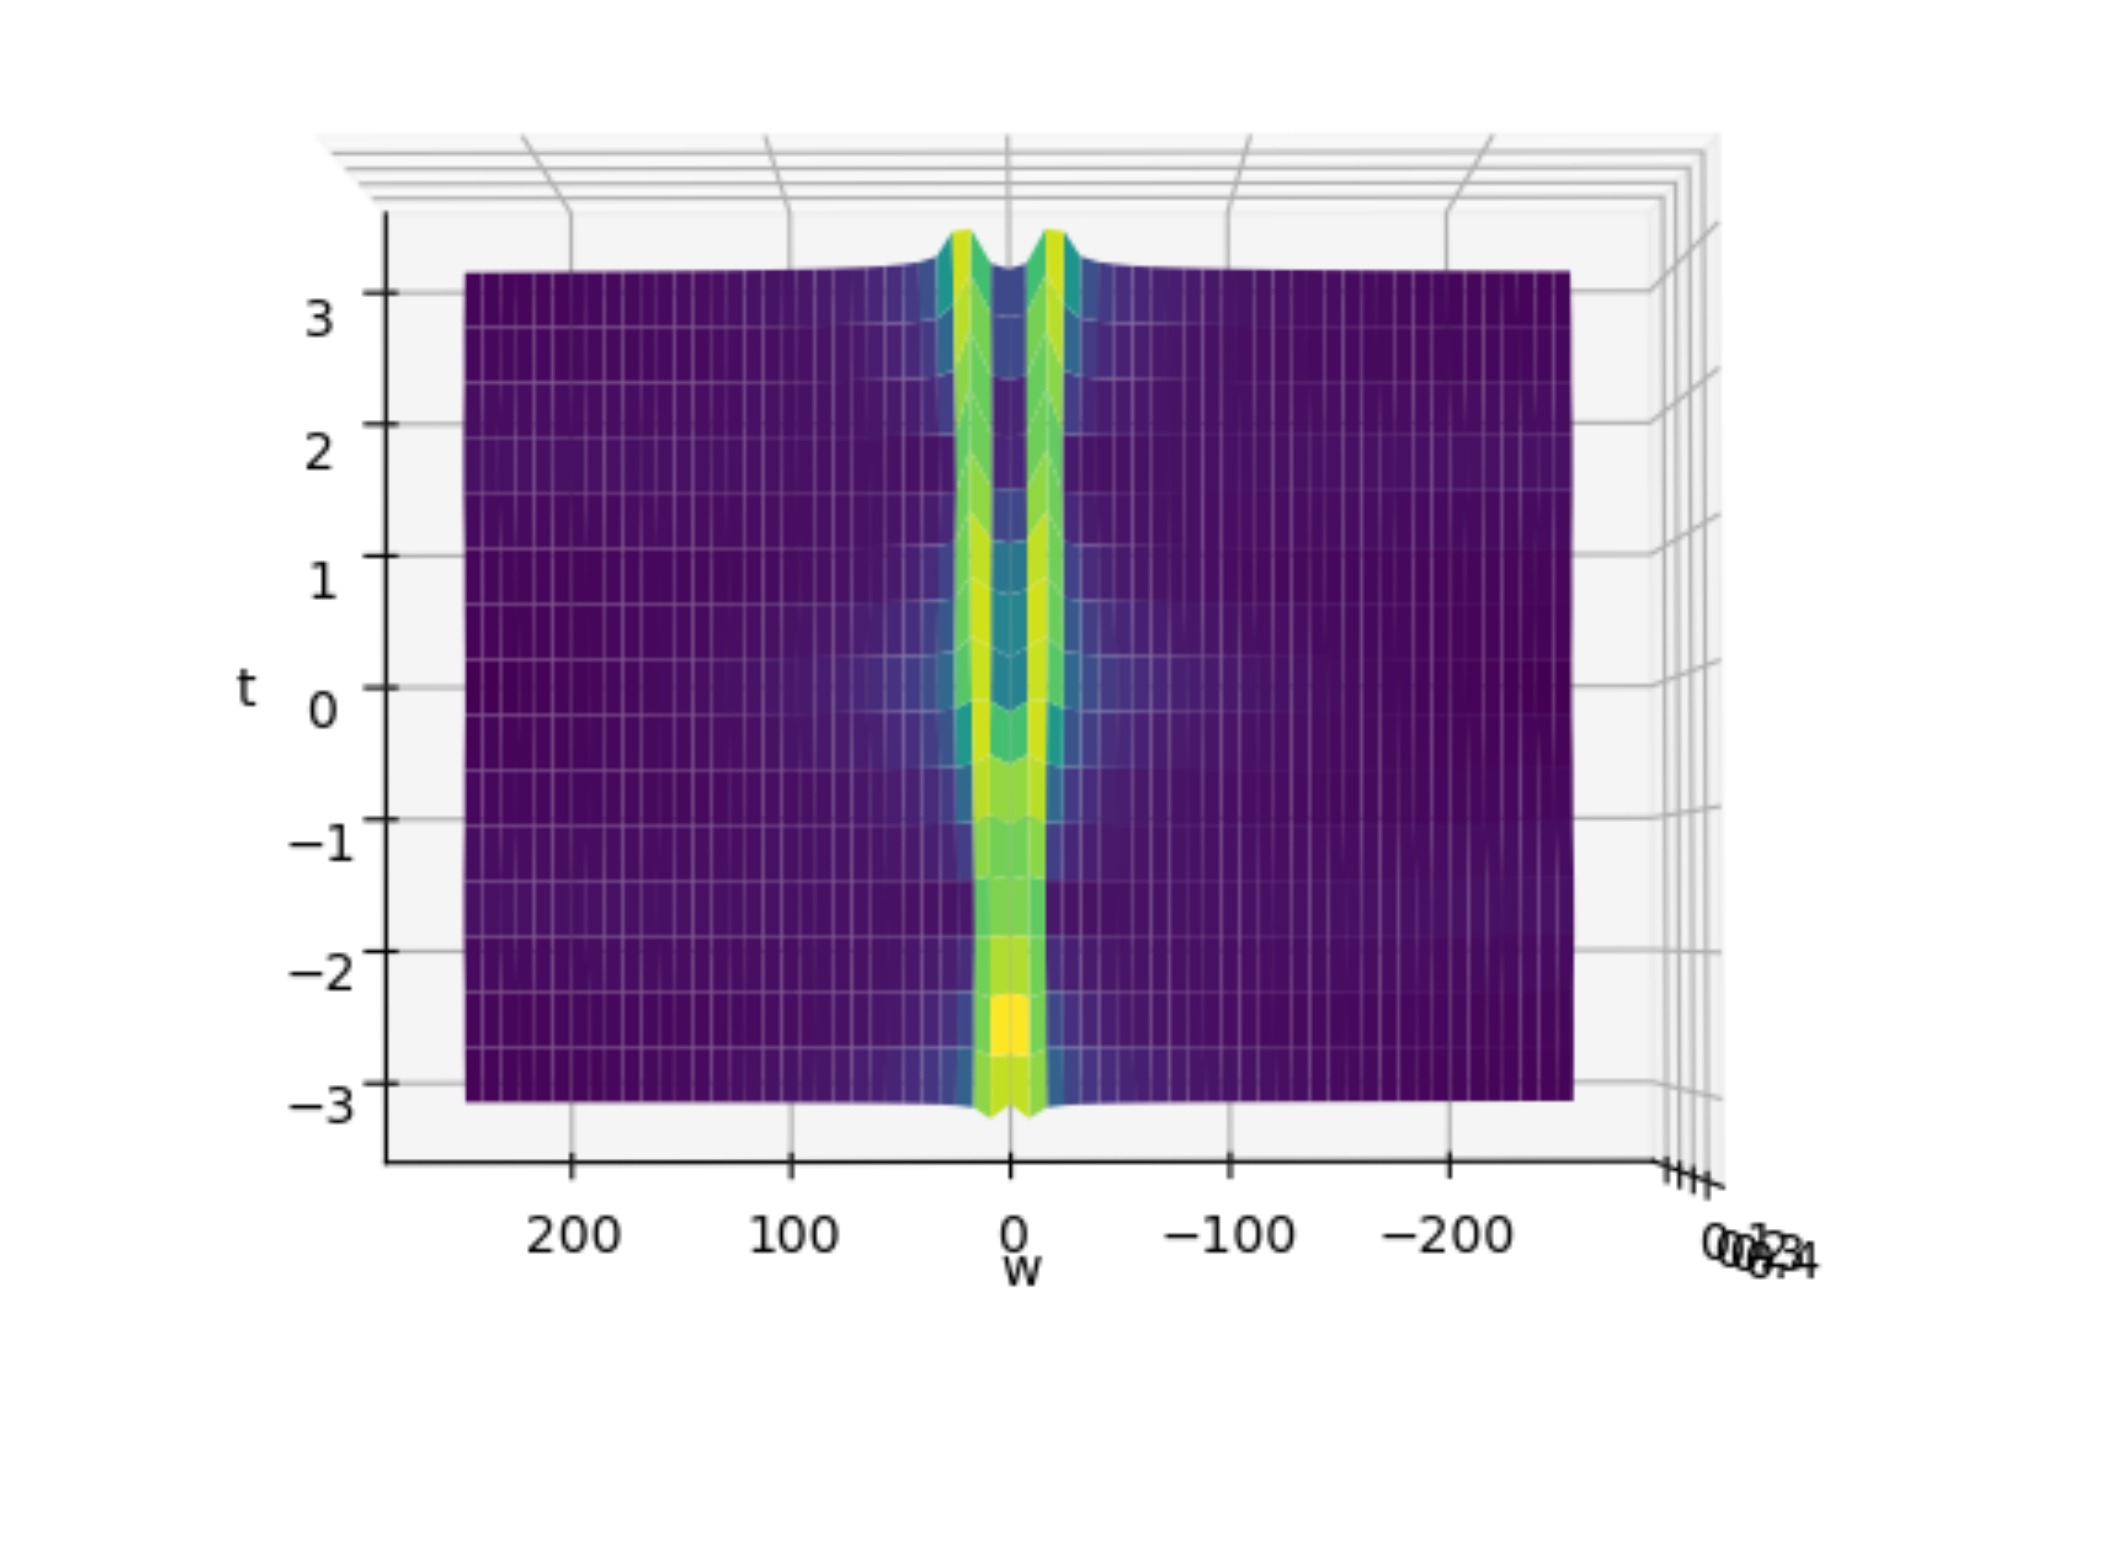
\includegraphics[scale=0.3]{Figure9.png}}\\
From the figures we can clearly see that the peaks are getting separated as time goes on.This represents different frequencies in the signal.\\

\chapter{Observations}
Asymmetric signals are not easy to deal with and we have to chose proper windows to get defined peaks in the spectrum. We saw that we do not get exact results when trying to estimate frequency of signals and with the added noise we get even worse results. \\We have to be careful in dealing with these signals and obtaining proper results. \\Sometimes it might be better to look at signals in time domain and we can obtain more information. The conclusion is that we can come up with intelligent ways in processing the signal better.\\

\end{document}












